\documentclass[tikz,border=3.14mm]{standalone}
\usetikzlibrary{automata,positioning,arrows.meta}

\begin{document}
    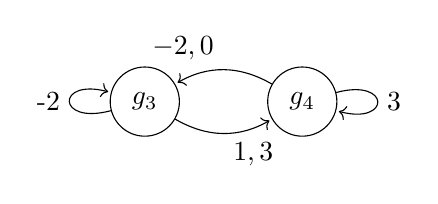
\begin{tikzpicture}[shorten >=1pt,node distance=2cm,on grid,auto] 
        \node[state] (q_0) {$g_3$};
        \node[state] (q_1) [right=of q_0] {$g_4$};
        \path[->]
        (q_0) edge[loop left] node{-2} ()
                edge[bend right] node[below right]{$1,3$} (q_1)
        (q_1) edge[bend right] node[above left]{$-2,0$} (q_0) 
                edge[loop right] node{3} ();
    \end{tikzpicture}
    
    Automaton recognizing the imaginary parts of points in $\partial \mathcal{K} \cap \Delta_{1,0,-1/5}$ in base $-4$.
\end{document}